\chapter{PID tuning as a multi-objective optimization method}
\label{chap:PIDMOOP}

%-----------------------------
\section{Solution of the multi-objective optimization tuning}
\label{sec:SolMOOP}
When solving the \gls{moop} presented in \eqref{eq:probmoo} for different normalized plants, one is able to find a family of Pareto fronts. The script used to find these fronts can be found in the companion software for this book\footnote{the script is named \texttt{GenerateParetosThreeFun.m}}.

Defining the normalized variable $\hat{s}=T s$, the time delay for the normalized plant, $\tau_0$, becomes:
\begin{equation}
\tau_0 = \frac{L}{T},
\label{eq:tauNorm}
\end{equation}
%
Then, one is able to find the corresponding Pareto front for the normalized plant, that represents many combinations of lag time and dead time. The gain of the plant is considered to be included in the controller gain for the sake of the normalization.

The steps that are required to find the front for each Pareto is presented in Algorithm~\ref{alg:GenerateParetos3}.
%
\begin{algorithm}[tb]
	\begin{algorithmic}
		\State $M_{svec} \gets [10,2,1.8,1.6,1.4]$
		\State $\tau_{0vec} \gets (0.1:0.1:2)$
		\State $a_{vec} \gets (0:0.1:1)$
		\ForAll{permutations of $M_s \in M_{svec}$, $\tau_0 \in \tau_{0vec}$ and $a \in a_{vec}$}
			\State Define the plant \gls{plan} with $\tau_{0}$ and $a$
			\State Find initial tuning  using Usort2 method
			\State Create cost function $J(\theta) = [J_{di}(\theta, \gls{plan}, t),J_{do}(\theta, \gls{plan}, t),J_{r}(\theta, \gls{plan}, t) ]$
			\State Create constraint function $MCalc(\theta, \gls{plan}) \leq M_s$
			\State Apply ENNC method to find the Pareto front
			\State Apply Pareto filter
			\State Compute actual $M_s$ for each controller
			\State Save to file
		\EndFor
	\end{algorithmic}
\caption{Script for finding all Pareto fronts.}
\label{alg:GenerateParetos3}
\end{algorithm}
%

The Pareto front was found for each normalized plant with approximately 1000 points for each front. Using the steps of Algorithm~\ref{alg:GenerateParetos3}, a total of 220 different normalized plants were considered. Also, five different values of desired maximum $M_s$ were considered. Therefore a total of 1100 different cases were computed. For each case, a Pareto was found using the ENNC method with approximately 500 points for each front. Notice that each of these points represents a different tuning (and since the optimization was done for \gls{2dof} controllers, each point has a different value for $\kappa_p$, $\tau_i$, $\tau_d$ and $\beta$), the total possible Pareto optimal \gls{pid} controllers found, reaches approximately 500 000 different controllers for all the totality of the plants and $M_s$. All these controller tunings, can also be found in the companion software of this book as comma separated values files.

\section{Viability for tuning rules}
\label{sec:TuningRulesMOOP}
In this section, an example of how to use the gathered data from the Pareto front is presented in order to find a tuning rule. The results that are presented here where first documented in \cite{Moya2017}.

For this particular example, the variable $a$ takes values from $0$ to $1$ in $0.1$ steps and $\tau_0$ takes values from $1$ to $2$ in $0.1$ steps and $M_{s,max}=2$. However, the complete set of data also has values for $\tau_0 < 1$.

The methodology after finding the data is to perform a curve fitting procedure to find equations useful to compute the value of $\kappa_p$, $\tau_i$, $\tau_d$ and $beta$ as a function of $a$ and $\tau_0$ and a factor of degradation of the cost functions.

Notice that the idea is that, knowing the model of the plant, the values of the controller parameters can be computed without needing to perform all the optimization, and also the decision maker can also select the weight for each cost function in order to find a single set of parameters.

This idea of "allowed degradation" is now introduced. Considered that $J_{di}$ and $J_{do}$ are normalized as:
%
\begin{align}
\delta &= \frac{J_{di}(\theta)-J_{di, min}(\theta)}{J_{di,max}(\theta)-J_{di,min}(\theta)},\label{eq:delta}\\
\gamma &= \frac{J_{do}(\theta)-J_{do, min}(\theta)}{J_{do,max}(\theta)-J_{do,min}(\theta)},\label{eq:gamma}
\end{align}
%
where both $0 \le \delta \le 1$ and $0 \le \gamma \le 1$. Then, these variables can be understood as the degradation of the function, considering the minimum value of the cost function as its optimal. Then a value of $\delta=1$ represents a degradation of 100\% of the $J_{di}$ cost function. It is important to notice that the Pareto front is constructed from three different cost functions. Therefore, if one select the value of the allowed degradation for two functions (in this case, $\delta$ and $\gamma$), the logical step is to choose the lowest value of $J_r$ that complies with the maximum degradation of the other two functions. Then for example,  if $\delta=\gamma=1$, which means that the decision maker is willing to allowed a complete degradation of $J_{di}$ and $J_{do}$, the resulting tuning is expected to represent the optimal tuning for servo control.

Now, it is important to understand that the ``degraded'' tuning, is also optimal in the Pareto sense, because all found tunings are optimal. Therefore, in these frame, a degraded tuning does not mean a ``bad'' tuning, it is just the result of a choice decision when selecting the final optimal controller. In all Pareto decisions, a compromise has to be made when selecting the final solution.

The work done to find the tuning rules, summed up to almost two hundred and twenty regressions for all values of $a$ and $\tau_0$ in order to find the complete set of parameters $\bm{\theta}$.

After different heuristic tests, the regression analysis showed that a second order fit gave the best results for $\kappa_p$, $\tau_i$ and $\tau_d$,  while  a first order fit for $\beta$ was enough to model the variation of this parameter. 

The tuning rule for all controller parameters are proposed to be as:  
%
\begin{align}
\kappa_p &= p_{00}+p_{01}\cdot\gamma+p_{02}\cdot\delta\nonumber\\
&\quad + p_{03}\cdot\gamma^2+p_{04}\cdot\gamma\cdot \delta+p_{05}\cdot\delta^2,\label{E:eqkp}\\
%
\tau_i &= p_{10}+p_{11}\cdot\gamma+p_{12}\cdot\delta\nonumber\\
&\quad + p_{13}\cdot\gamma^2+p_{14}\cdot\gamma\cdot \delta+p_{15}\cdot\delta^2,\label{E:eqTi}\\
%
\tau_d &= p_{20}+p_{21}\cdot\gamma+p_{22}\cdot\delta\nonumber\\
&\quad+p_{23}\cdot\gamma^2+p_{24}\cdot\gamma\cdot \delta+p_{25}\cdot\delta^2,\label{E:eqTd}\\
%
\beta &=p_{30}+p_{31}\cdot\gamma+p_{32}\cdot\delta,\label{E:eqbeta}
\end{align}
%

The coefficients $p_{ij}$, where $i=\{0,1,2,3\}$ and $j=\{0,1,2,3,4,5\}$, depend on $a$ and $\tau_0$. The corresponding fits of $\kappa_p$, $\tau_i$, $\tau_d$ and $\beta$, are shown in Fig.~\ref{F:cftoolkp}. \ref{F:cftoolTi}, \ref{F:cftoolTd} and \ref{F:cftoolbeta} for $a=0.1$ and $\tau_{0}=1$.   % a second order surface was found to be the best fit for all eleven fits overall, as shown in figure \ref{F:firstfit}.
%
\begin{figure}[tb]
	\centering
	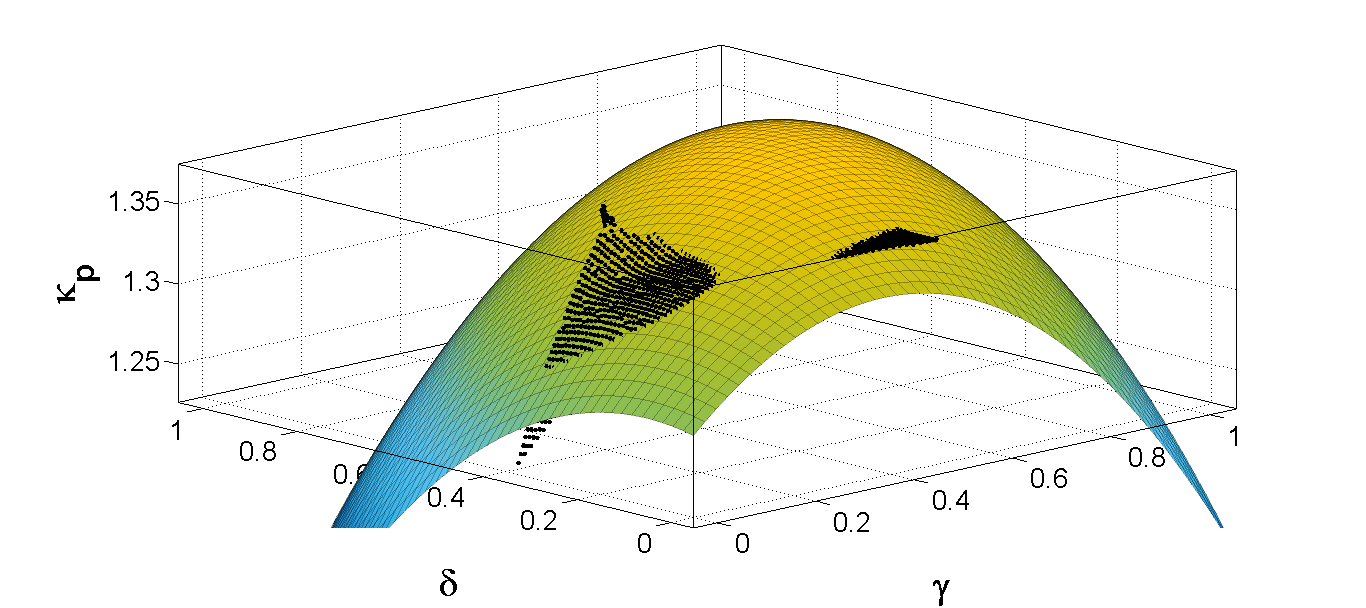
\includegraphics[width=\columnwidth]{kpfit2.png}
	\caption{Second order fit for $\kappa_p$ when $a=0.1$ and $\tau_{0}=1$}
	\label{F:cftoolkp}
\end{figure}
%
\begin{figure}[tb]
	\centering
	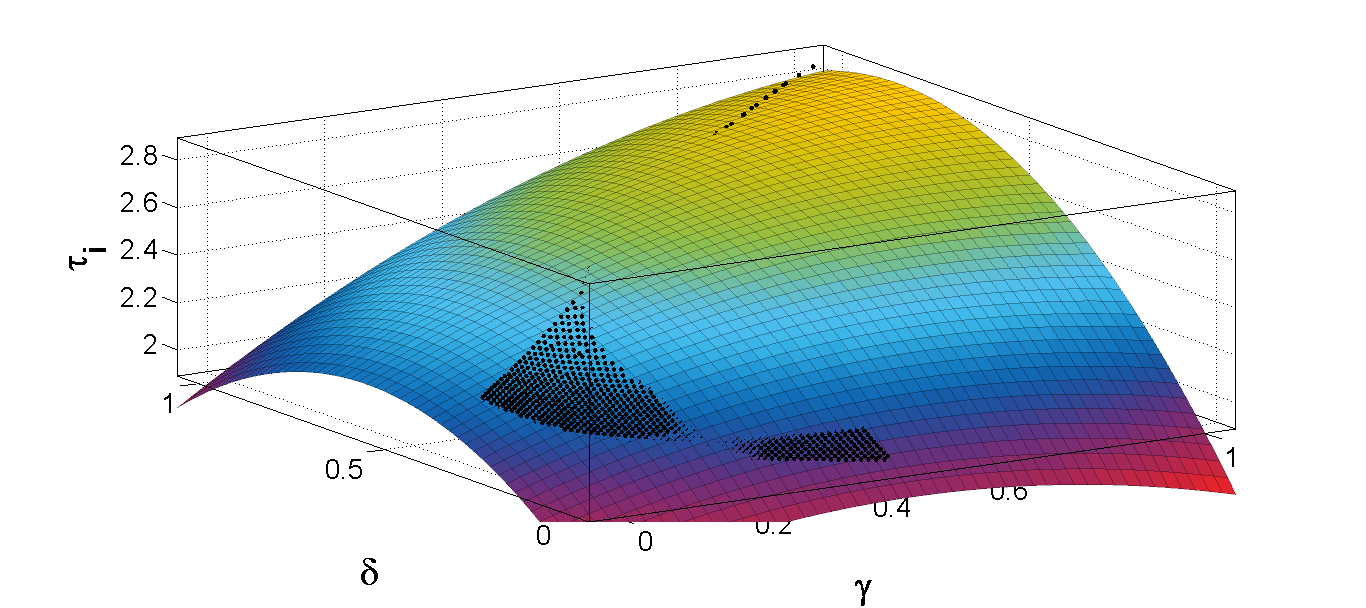
\includegraphics[width=\columnwidth]{Tifit2.png}
	\caption{Second order fit for $\tau_i$ when $a=0.1$ and $\tau_0=1$}
	\label{F:cftoolTi}
\end{figure}
%
\begin{figure}[tb]
	\centering
	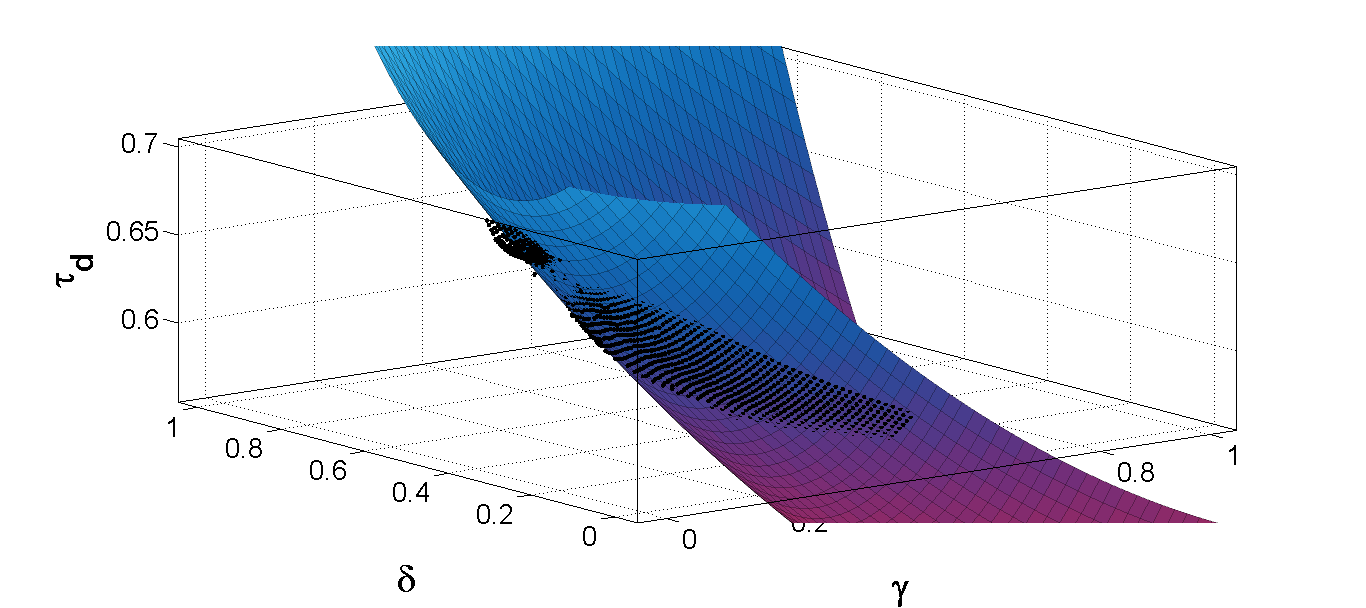
\includegraphics[width=0.5\textwidth]{Tdfit2.png}
	\caption{Second order fit for $\tau_d$ when $a=0.1$ and $\tau_0=1$}
	\label{F:cftoolTd}
\end{figure}
%
\begin{figure}[tb]
	\centering
	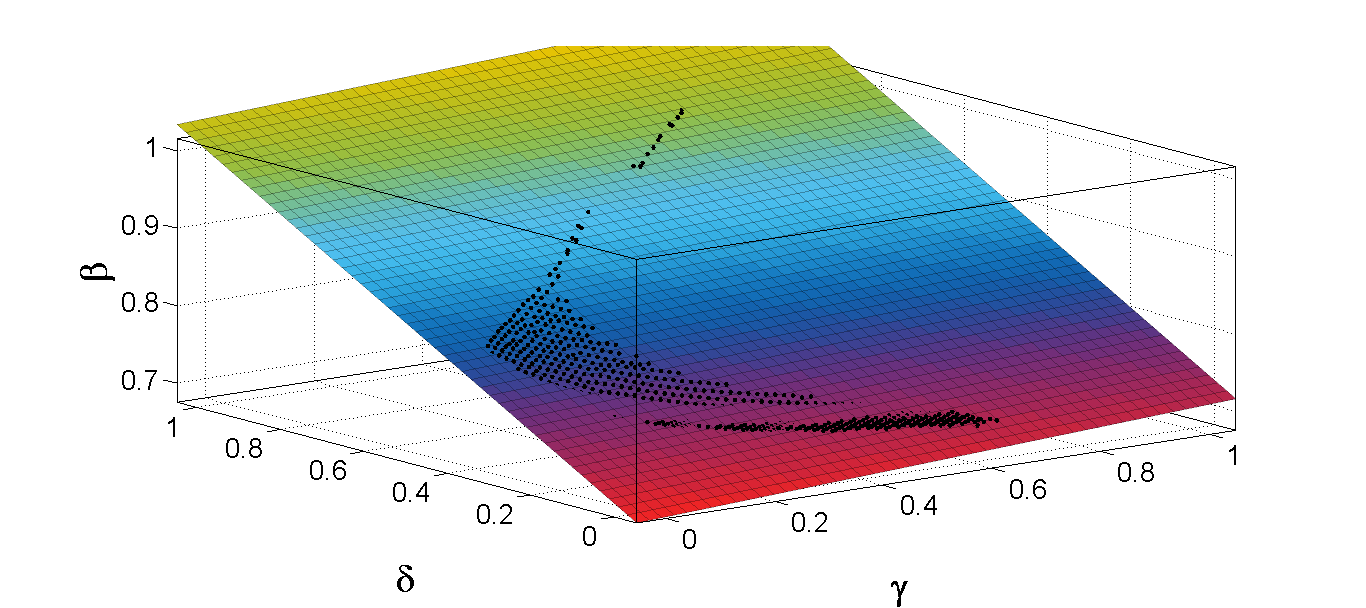
\includegraphics[width=0.5\textwidth]{betafit2.png}
	\caption{First order fit for $\beta$ when $a=0.1$ and $\tau_0=1$}
	\label{F:cftoolbeta}
\end{figure}

It is important to notice an important caveat. In those figures, the values that belong to the computed Pareto are shown as dots, while the corresponding regression is ploted as a 3D surface. It can be noticed that the domain of the regressions is larger than the actual results of the Pareto. Even thought the fitting is good (around $R=0.9$), the regression represents interpolation and extrapolation from the real data. Therefore, it is important too check how well the regression works and to not exceed the limits where it yields good results.

Going back to the $p_{ij}$, it has to be notice that the value of these parameters, depends on the model of the plant. Therefore, it is required to find another set of regressions over these parameters in terms of $a$ and $\tau_0$. Therefore, a curve fitting procedure is also required for each $p_{ij}$. As an example of these regressions, 
%
\begin{figure}[tb]
	\centering
	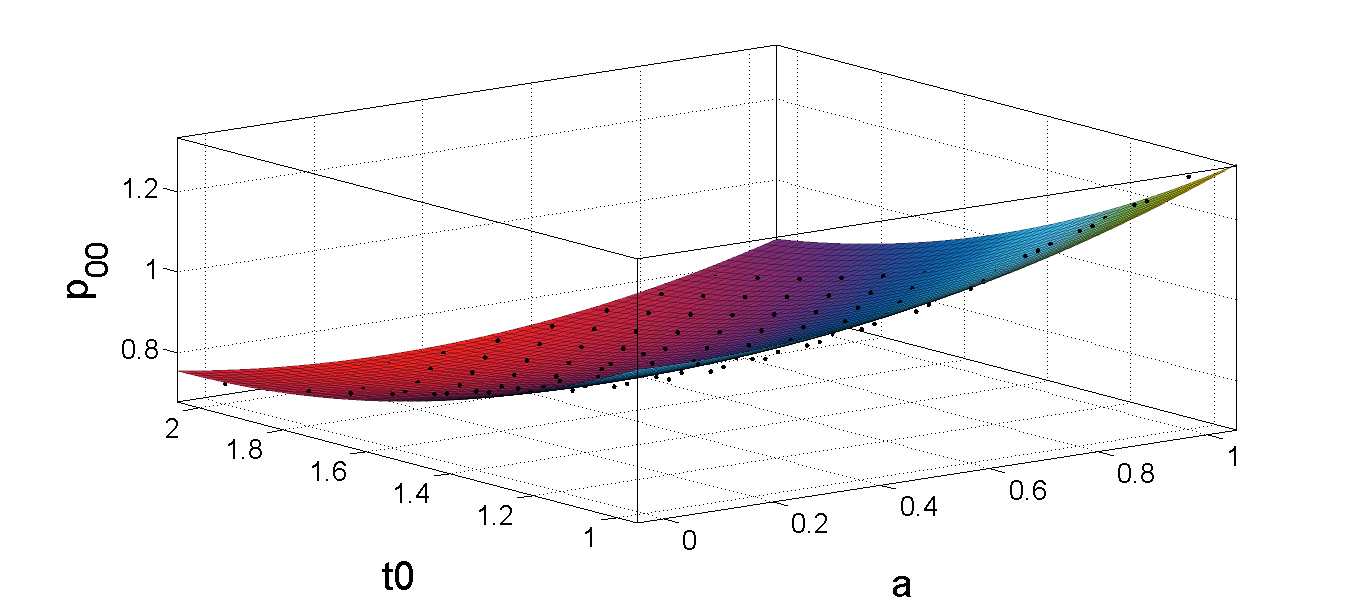
\includegraphics[width=0.5\textwidth]{./a00fit2.png}
	\caption{Second order fit for $p_{00}$ in $\kappa_p$}
	\label{F:coeff}
\end{figure}
%
Fig.~\ref{F:coeff} shows the result for $p_{00}$ parameter as a function of $a$ and $\tau_0$. The selected fit for every coefficient in the range of $1\leq \tau_0 \leq2$, was also a second order polinomial. The equation that is considered has the form:
%
\begin{equation}
p_{ij} = b_{j0}+b_{j1}a+b_{j2} \tau_0+b_{j3}a^2+b_{j4}a \tau_0+b_{j5}\tau_0^2 .
\label{E:coeff}
\end{equation}

Another two hundred and twenty regressions were made for all $p_{ij}$. The results for every coefficient are shown in Table~\ref{T:T1} for $kappa_p$, Table~\ref{T:ti} for the integral time, Table~\ref{T:td} for the derivative time and Table~\ref{T:beta} for $\beta$.

% Please add the following required packages to your document preamble:
% \usepackage{multirow}
%\begin{table}
%\centering
%\caption{Parameters for $\kappa_p$.}
%\label{T:T1}
%\begin{tabular}{|c|l|l|}
%\hline
%\multicolumn{3}{|c|}{$\kappa_p$ coefficients}           \\ \hline
%$p_{ij}$                  & \multicolumn{2}{c|}{$b_{ik}$} \\ \hline
%\multirow{6}{*}{$p_{00}$} & $b_{00}$      & 1.8203        \\ \cline{2-3} 
%                     & $b_{01}$      & 0.12765       \\ \cline{2-3} 
%                     & $b_{02}$      & -1.0484       \\ \cline{2-3} 
%                     & $b_{03}$      & 0.27085       \\ \cline{2-3} 
%                     & $b_{04}$      & -0.15141      \\ \cline{2-3} 
%                     & $b_{05}$      & 0.25505       \\ \hline
%\multirow{6}{*}{$p_{01}$} & $b_{10}$      & 0.32832       \\ \cline{2-3} 
%                     & $b_{11}$      & 0.22439       \\ \cline{2-3} 
%                     & $b_{12}$      & -0.26761      \\ \cline{2-3} 
%                     & $b_{13}$      & -0.022374     \\ \cline{2-3} 
%                     & $b_{14}$      & -0.068708     \\ \cline{2-3} 
%                     & $b_{15}$      & 0.076273      \\ \hline
%\multirow{6}{*}{$p_{02}$} & $b_{20}$      & 0.29122       \\ \cline{2-3} 
%                     & $b_{21}$      & -0.12878      \\ \cline{2-3} 
%                     & $b_{22}$      & -0.25003      \\ \cline{2-3} 
%                     & $b_{23}$      & 0.10461       \\ \cline{2-3} 
%                     & $b_{24}$      & 0.0048329     \\ \cline{2-3} 
%                     & $b_{25}$      & 0.059478      \\ \hline
%\multirow{6}{*}{$p_{03}$} & $b_{30}$      & 0.042733      \\ \cline{2-3} 
%                     & $b_{31}$      & -0.52048      \\ \cline{2-3} 
%                     & $b_{32}$      & -0.25437      \\ \cline{2-3} 
%                     & $b_{33}$      & 0.47345       \\ \cline{2-3} 
%                     & $b_{34}$      & -0.11069      \\ \cline{2-3} 
%                     & $b_{35}$      & 0.078691      \\ \hline
%\multirow{6}{*}{$p_{04}$} & $b_{40}$      & -0.077455     \\ \cline{2-3} 
%                     & $b_{41}$      & 0.61083       \\ \cline{2-3} 
%                     & $b_{42}$      & 0.24951       \\ \cline{2-3} 
%                     & $b_{43}$      & -0.60316      \\ \cline{2-3} 
%                     & $b_{44}$      & 0.19685       \\ \cline{2-3} 
%                     & $b_{45}$      & -0.071314     \\ \hline
%\multirow{6}{*}{$p_{05}$} & $b_{50}$      & -0.41226      \\ \cline{2-3} 
%                     & $b_{51}$      & -0.24733      \\ \cline{2-3} 
%                     & $b_{52}$      & 0.29554       \\ \cline{2-3} 
%                     & $b_{53}$      & 0.080236      \\ \cline{2-3} 
%                     & $b_{54}$      & 0.013411      \\ \cline{2-3} 
%                     & $b_{55}$      & -0.091089     \\ \hline
%\end{tabular}
%\end{table}
%
\begin{table}[tb]
	\centering
	\caption{Coefficients for $\kappa_p$.}
	\label{T:T1}
	\begin{tabular}{@{}cll|cll@{}}
		\hline
		%\multicolumn{6}{c}{$\kappa_p$ coefficients}           \\ \hline
		$p_{ij}$                  & \multicolumn{2}{c}{$b_{ik}$} & $p_{ij}$ & \multicolumn{2}{c}{$b_{ik}$}\\
		\hline
		\multirow{6}{*}{$p_{00}$} & $b_{00}$  & $1.820$ &   \multirow{6}{*}{$p_{01}$} & $b_{10}$ & $0.328$ \\ % \cline{2-3} \cline{5-6}
		& $b_{01}$      & $0.128$   &  	& $b_{11}$      & $0.224$ \\ % \cline{2-3} \cline{5-6}
		& $b_{02}$      & $-1.048$   &	& $b_{12}$      & $-0.268$ \\ % \cline{2-3} \cline{5-6}
		& $b_{03}$      & $0.270$   &	& $b_{13}$      & $-0.022$ \\ % \cline{2-3} \cline{5-6}
		& $b_{04}$      & $-0.151$  & 	& $b_{14}$      & $-0.069$  \\ % \cline{2-3} \cline{5-6}
		& $b_{05}$      & $0.255$   &	& $b_{15}$      & $0.076$    \\ \hline
		%
		\multirow{6}{*}{$p_{02}$} & $b_{20}$  & $0.291$	& \multirow{6}{*}{$p_{03}$} & $b_{30}$ & $0.043$ \\ % \cline{2-3} \cline{5-6}
		& $b_{21}$      & $-0.129$   & & $b_{31}$      & $-0.520$  \\ % \cline{2-3} \cline{5-6}
		& $b_{22}$      & $-0.250$   & & $b_{32}$      & $-0.254$  \\ % \cline{2-3} \cline{5-6}
		& $b_{23}$      & $0.105$    & & $b_{33}$      & $0.473$   \\ % \cline{2-3} \cline{5-6}
		& $b_{24}$      & $0.005$  & & $b_{34}$      & $-0.111$  \\ % \cline{2-3} \cline{5-6}
		& $b_{25}$      & $0.059$   & & $b_{35}$      & $0.079$  \\ \hline
		%
		\multirow{6}{*}{$p_{04}$} & $b_{40}$      & $-0.077$  & \multirow{6}{*}{$p_{05}$} & $b_{50}$      & $-0.412$   \\ %\cline{2-3} \cline{5-6}
		& $b_{41}$      & $0.611$     &  & $b_{51}$      & $-0.247$\\ %\cline{2-3} \cline{5-6}
		& $b_{42}$      & $0.249$     &  & $b_{52}$      & $0.296$\\ % \cline{2-3} \cline{5-6}
		& $b_{43}$      & $-0.603$    &  & $b_{53}$      & $0.080$\\ %\cline{2-3} \cline{5-6}
		& $b_{44}$      & $0.197$     &  & $b_{54}$      & $0.013$\\ % \cline{2-3} \cline{5-6}
		& $b_{45}$      & $-0.071$   &  & $b_{55}$      & $-0.091$\\
		\hline
	\end{tabular}
\end{table}
%
\begin{table}[tb]
	\centering
	\caption{Coefficients for $\tau_i$.}
	\label{T:ti}
	\begin{tabular}{@{}cll|cll@{}}
		\hline
		%\multicolumn{6}{c}{$\kappa_p$ coefficients}           \\ \hline
		$p_{ij}$                  & \multicolumn{2}{c}{$b_{ik}$} & $p_{ij}$ & \multicolumn{2}{c}{$b_{ik}$}\\
		\hline
		\multirow{6}{*}{$p_{10}$} & $b_{00}$  & $0.591$
		&   \multirow{6}{*}{$p_{11}$} & $b_{10}$ & $-0.408$
		\\ % \cline{2-3} \cline{5-6}
		& $b_{01}$      & $0.559$   &  	& $b_{11}$      & $0.640$ \\ % \cline{2-3} \cline{5-6}
		& $b_{02}$      & $0.545$   &	& $b_{12}$      & $0.855$ \\ % \cline{2-3} \cline{5-6}
		& $b_{03}$      & $0.017$   &	& $b_{13}$      & $-0.238$ \\ % \cline{2-3} \cline{5-6}
		& $b_{04}$      & $0.045$  & 	& $b_{14}$      & $-0.0024$  \\ % \cline{2-3} \cline{5-6}
		& $b_{05}$      & $-0.028$   &	& $b_{15}$      & $-0.193$    \\ \hline
		%
		\multirow{6}{*}{$p_{12}$} & $b_{20}$  & $1.718$
		& \multirow{6}{*}{$p_{13}$} & $b_{30}$ & $1.297$ \\ % \cline{2-3} \cline{5-6}
		& $b_{21}$      & $0.652$   & & $b_{31}$      & $-0.423$  \\ % \cline{2-3} \cline{5-6}
		& $b_{22}$      & $-1.160$   & & $b_{32}$      & $-2.095$  \\ % \cline{2-3} \cline{5-6}
		& $b_{23}$      & $-0.855$    & & $b_{33}$      & $1.226$   \\ % \cline{2-3} \cline{5-6}
		& $b_{24}$      & $-0.719$  & & $b_{34}$      & $-1.041$  \\ % \cline{2-3} \cline{5-6}
		& $b_{25}$      & $0.363$   & & $b_{35}$      & $0.649$  \\ \hline
		%
		\multirow{6}{*}{$p_{14}$} & $b_{40}$      & $-0.077$  & \multirow{6}{*}{$p_{15}$} & $b_{50}$      & $-1.346$   \\ %\cline{2-3} \cline{5-6}
		& $b_{41}$      & $0.621$     &  & $b_{51}$      & $-1.148$\\ %\cline{2-3} \cline{5-6}
		& $b_{42}$      & $0.277$     &  & $b_{52}$      & $1.224$\\ % \cline{2-3} \cline{5-6}
		& $b_{43}$      & $-1.193$    &  & $b_{53}$      & $-0.218$\\ %\cline{2-3} \cline{5-6}
		& $b_{44}$      & $1.030$     &  & $b_{54}$      & $0.512$\\ % \cline{2-3} \cline{5-6}
		& $b_{45}$      & $-0.025$   &  & $b_{55}$      & $-0.572$\\
		\hline
	\end{tabular}
\end{table}
%
\begin{table}[tb]
	\centering
	\caption{Coefficients for $\tau_d$.}
	\label{T:td}
	\begin{tabular}{@{}cll|cll@{}}
		\hline
		%\multicolumn{6}{c}{$\kappa_p$ coefficients}           \\ \hline
		$p_{ij}$                  & \multicolumn{2}{c}{$b_{ik}$} & $p_{ij}$ & \multicolumn{2}{c}{$b_{ik}$}\\
		\hline
		\multirow{6}{*}{$p_{20}$} & $b_{00}$  & $0.111$
		&   \multirow{6}{*}{$p_{21}$} & $b_{10}$ & $-0.0076$
		\\ % \cline{2-3} \cline{5-6}
		& $b_{01}$      & $0.450$   &  	& $b_{11}$      & $-0.163$ \\ % \cline{2-3} \cline{5-6}
		& $b_{02}$      & $0.274$   &	& $b_{12}$      & $-0.212$ \\ % \cline{2-3} \cline{5-6}
		& $b_{03}$      & $-0.025$   &	& $b_{13}$      & $0.154$ \\ % \cline{2-3} \cline{5-6}
		& $b_{04}$      & $-0.069$  & 	& $b_{14}$      & $-0.074$  \\ % \cline{2-3} \cline{5-6}
		& $b_{05}$      & $0.003$   &	& $b_{15}$      & $0.0026$    \\ \hline
		%
		\multirow{6}{*}{$p_{22}$} & $b_{20}$  & $-0.238$	& \multirow{6}{*}{$p_{23}$} & $b_{30}$ & $-0.237$ \\ % \cline{2-3} \cline{5-6}
		& $b_{21}$      & $0.105$   & & $b_{31}$      & $-0.938$  \\ % \cline{2-3} \cline{5-6}
		& $b_{22}$      & $-0.016$   & & $b_{32}$      & $1.121$  \\ % \cline{2-3} \cline{5-6}
		& $b_{23}$      & $-0.234$    & & $b_{33}$      & $0.496$   \\ % \cline{2-3} \cline{5-6}
		& $b_{24}$      & $0.094$  & & $b_{34}$      & $0.331$  \\ % \cline{2-3} \cline{5-6}
		& $b_{25}$      & $-0.0254$   & & $b_{35}$      & $-0.641$  \\ \hline
		%
		\multirow{6}{*}{$p_{24}$} & $b_{40}$      & $0.379$  & \multirow{6}{*}{$p_{25}$} & $b_{50}$      & $-0.224$   \\ %\cline{2-3} \cline{5-6}
		& $b_{41}$      & $0.908$     &  & $b_{51}$      & $0.109$\\ %\cline{2-3} \cline{5-6}
		& $b_{42}$      & $-1.330$     &  & $b_{52}$      & $0.805$\\ % \cline{2-3} \cline{5-6}
		& $b_{43}$      & $-1.203$    &  & $b_{53}$      & $0.669$\\ %\cline{2-3} \cline{5-6}
		& $b_{44}$      & $0.215$     &  & $b_{54}$      & $-0.527$\\ % \cline{2-3} \cline{5-6}
		& $b_{45}$      & $0.683$   &  & $b_{55}$      & $-0.112$\\
		\hline
	\end{tabular}
\end{table}
%
\begin{table}[tb]
	\centering
	\caption{Coefficients for $\beta$.}
	\label{T:beta}
	\begin{tabular}{@{}cll}
		\hline
		%\multicolumn{6}{c}{$\kappa_p$ coefficients}           \\ \hline
		$p_{ij}$                  & \multicolumn{2}{c}{$b_{ik}$}  \\
		\hline
		\multirow{6}{*}{$p_{30}$} & $b_{00}$  & $0.538$
		
		\\ % \cline{2-3} \cline{5-6}
		& $b_{01}$      & $0.023$     \\ % \cline{2-3} \cline{5-6}
		& $b_{02}$      & $0.179$   	\\ % \cline{2-3} \cline{5-6}
		& $b_{03}$      & $-0.114$    \\ % \cline{2-3} \cline{5-6}
		& $b_{04}$      & $0.047$   	  \\ % \cline{2-3} \cline{5-6}
		& $b_{05}$      & $-0.034$   \\ \hline
		%
		\multirow{6}{*}{$p_{31}$} & $b_{10}$  & -0.152
		\\ % \cline{2-3} \cline{5-6}
		& $b_{11}$      & $0.065$    \\ % \cline{2-3} \cline{5-6}
		& $b_{12}$      & $0.277$      \\ % \cline{2-3} \cline{5-6}
		& $b_{13}$      & $0.017$      \\ % \cline{2-3} \cline{5-6}
		& $b_{14}$      & $-0.052$   \\ % \cline{2-3} \cline{5-6}
		& $b_{15}$      & $-0.082$     \\ \hline
		%
		
		\multirow{6}{*}{$p_{32}$} & $b_{20}$  & 0.585
		\\ % \cline{2-3} \cline{5-6}
		& $b_{21}$      & $-0.082$    \\ % \cline{2-3} \cline{5-6}
		& $b_{22}$      & $-0.280$      \\ % \cline{2-3} \cline{5-6}
		& $b_{23}$      & $0.116$      \\ % \cline{2-3} \cline{5-6}
		& $b_{24}$      & $0.011$   \\ % \cline{2-3} \cline{5-6}
		& $b_{25}$      & $0.044$     \\ \hline
		%	
	\end{tabular}
\end{table}
%
\subsection{Comparison of regression against Pareto data}
%
To compare the results from the tuning rule, some simulations were done to compare the original data against the results. The plant model is: 

\begin{equation}
P_1(s) = \frac{e^{-1.5\hat{s}}}{(\hat{s}+1)(0.5\hat{s}+1)}
\label{E:P1}
\end{equation}

Where $K=1$, $T=1$~s, $L=1.5$~s and $a = 0.5$. Table \ref{T:comparison} compares the results of the optimization against the results of using the proposed tuning rule. Arbitrarily, the values for $\delta$ and $\gamma$ were chosen as $\delta=1$ and $\gamma=1$. 
%
\begin{table}[tb]
	\centering
	\caption{Result comparative of the Pareto data against the fitted data, with $\delta = 1$ and $\gamma = 1$.}
	\label{T:comparison}
	\begin{tabular}{@{}K{0.25\columnwidth} K{0.25\columnwidth} K{0.25\columnwidth}@{}}
		\toprule
		$\bm{\theta}$ and cost functions & From Pareto & From Tuning rule\\
		\midrule
		$\kappa_p$	& $0.810$	& $0.793$ \\
		$\tau_i$	& $2.176$~s	& $2.113$~s	\\
		$\tau_d$	& $0.644$~s	& $0.720$~s \\
		$\beta$		& $1.000$	& $1.000$ \\
		$J_r$		& $2.689$ 	& $2.691$ \\
		$J_{di}$ 	& $2.687$ 	& $2.673$ \\
		$J_{do}$	& $2.689$	& $2.691$ \\
		$M_s$		& $1.9174$	& $1.9449$\\
		\bottomrule
	\end{tabular}
\end{table} 

From Table~\ref{T:comparison}, can be seen that the results obtained from the  tuning rule are close to those obtained directly from the Pareto. Plots for each method were drawn as shown in Fig.~\ref{F:firstsim}.
%%%ESTA FIGURA HAY QUE CENTRARLA MEJOR
%
\begin{figure}[tb]
	\centering
	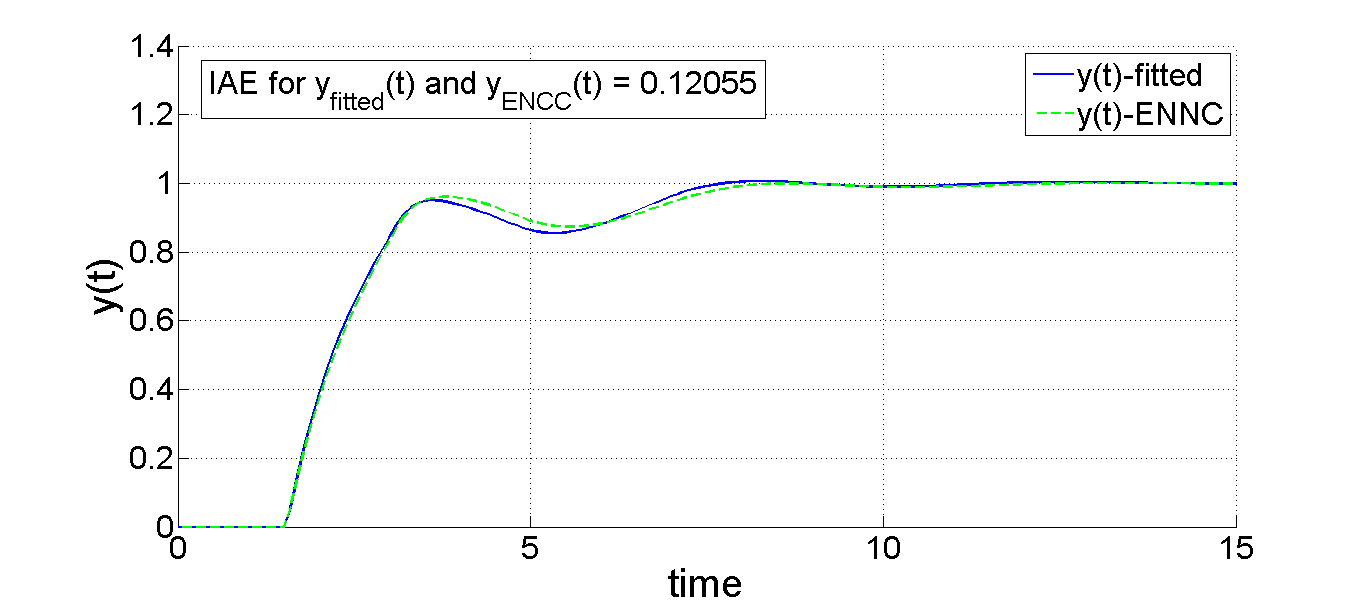
\includegraphics[width=0.8\columnwidth]{servo2.png}
	\caption{Servo response for the Pareto results found with the \gls{nnc} method and the tuning results.}
	\label{F:firstsim}
\end{figure}
%
The step response of the control signal is shown in Figure~\ref{F:u1} while the comparison for an input-disturbance is presented in Figure~\ref{F:di1} and for the output disturbance is in Figure~\ref{F:do1}. 
%
\begin{figure}[tb]
	\centering
	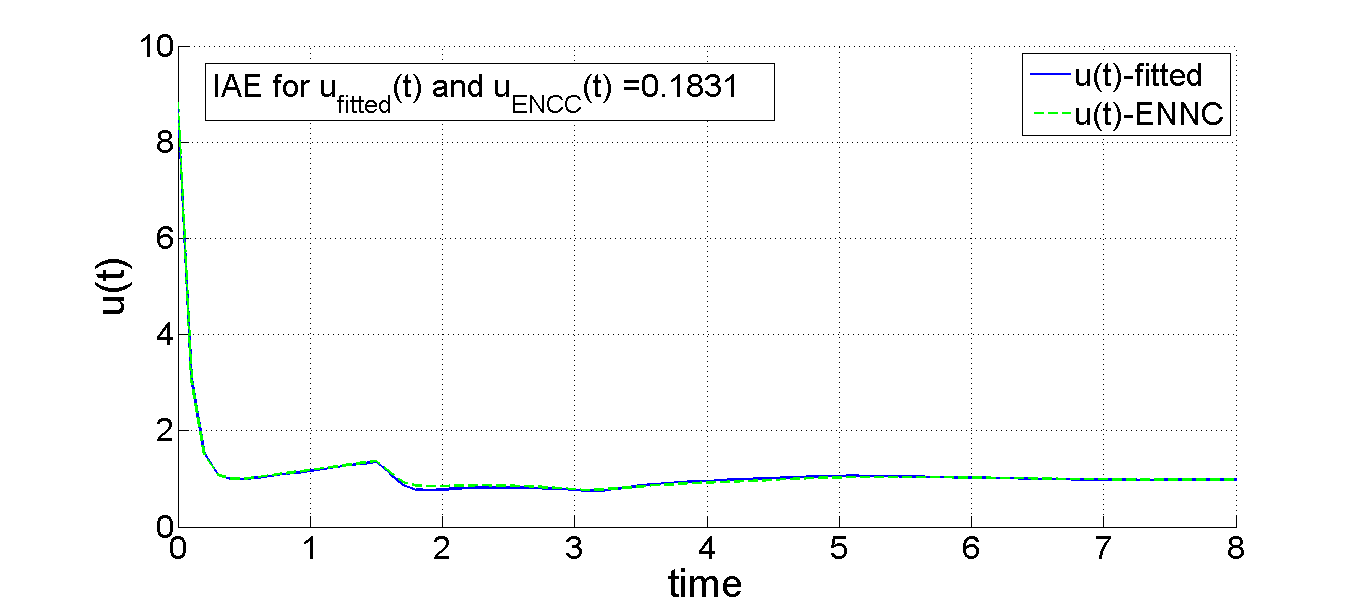
\includegraphics[width=0.8\columnwidth]{u2.png}
	\caption{Comparison of the control action  signal for a setpoint step change using the data from the Pareto found with the \gls{ennc} method and the tuning rule.}
	\label{F:u1}
\end{figure}
%
\begin{figure}[tb]
	\centering
	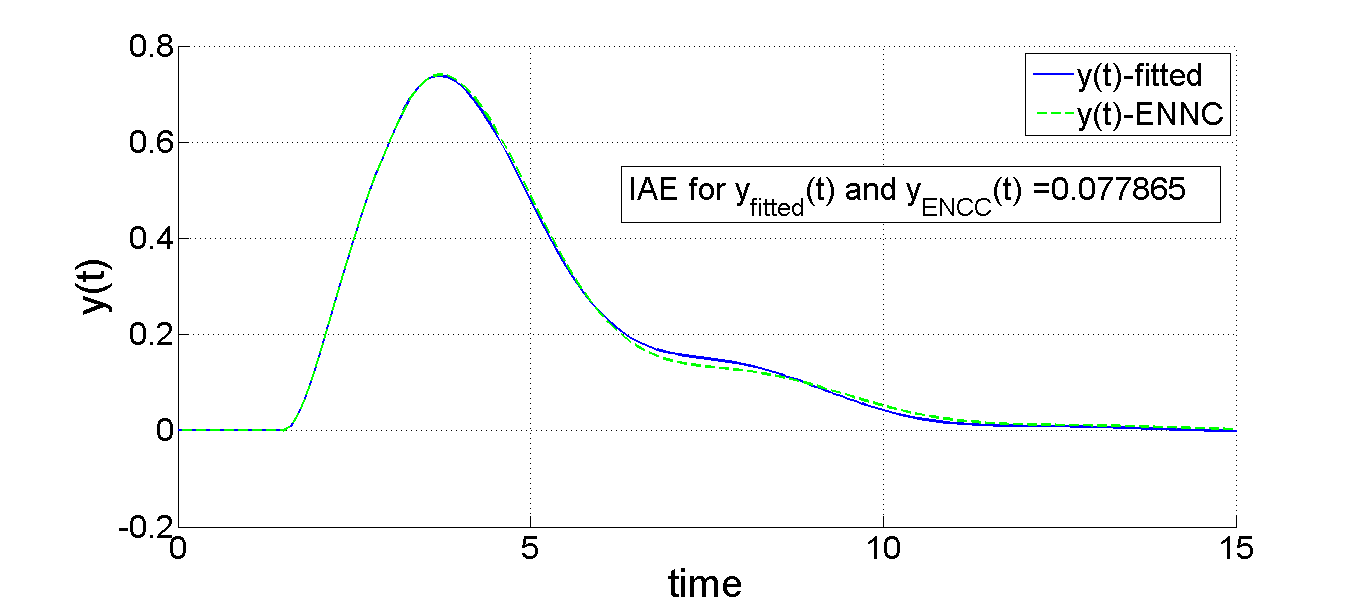
\includegraphics[width=0.8\columnwidth]{di2.png}
	\caption{Step input disturbance response for tuning from Pareto (ENNC method) and regressions results.}
	\label{F:di1}
\end{figure}
%
\begin{figure}[tb]
	\centering
	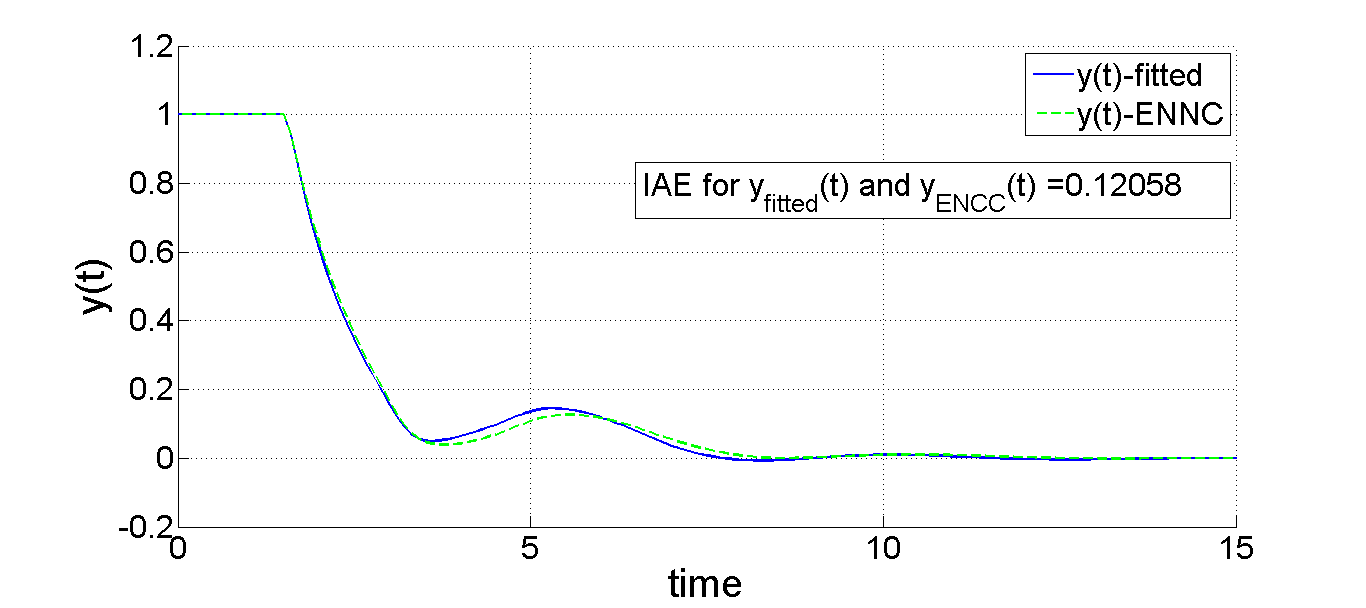
\includegraphics[width=0.8\columnwidth]{do2.png}
	\caption{Step output disturbance response for ENNC results and regressions results.}
	\label{F:do1}
\end{figure}
%
The figures show the \gls{iae} between both signals as a measure of how good the tuning rule approximates the optimization. As it can be seen, the responses are almost identical, showing that this methodology is feasible.

The tuning rule is also used for the extreme cases of $\tau_0$, that is, $\tau_0=1$ and $\tau_0=2$, using the following models:
%
\begin{equation}
P_F(\hat{s}) = \frac{e^{-\hat{s}}}{(\hat{s}+1)(0.5\hat{s}+1)},
\label{E:p2}
\end{equation}
%
\begin{equation}
P_S(\hat{s}) = \frac{e^{-2\hat{s}}}{(\hat{s}+1)(0.5\hat{s}+1)},
\label{E:p3}
\end{equation}
%
where $P_F(\hat{s})$ and $P_S(\hat{s})$ stand for the minimum and maximum  dead time considered in this study, respectively.

The allowed degradation was set to $\delta = 0.5$ and $\gamma = 0.5$. As before, one would expect to have the best servo response that complies with the allowed degradation. The comparison between the Pareto optimizations and the tuning rule for $P_F$ and $P_S$ are shown in Table~\ref{T:T2} and Table~\ref{T:T3} respectively.
%
\begin{table}[tb]
	\centering
	\caption{Results for $J_{di}$, $J_{do}$ and $J_{r}$, using $\delta = 0.5$ and $\gamma = 0.5$ for $P_F(s)$.}
	\label{T:T2}
	\begin{tabular}{@{}K{0.2\columnwidth} K{0.2\columnwidth} K{0.2\columnwidth} K{0.2\columnwidth}@{}}
		\toprule
		$\bm{\theta}$ and IAE & From tuning rule & From Pareto & Difference (\%)\\
		\midrule
		$\kappa_p$	& $1.150$ 	& $1.120$ & $2.67$\\
		$\tau_i$ 	& $1.987$ s & $1.900$ s & $4.58$\\
		$\tau_d$ 	& $0.425$ s & $0.495$ s & $-14.14$\\
		$\beta$ 	& $0.887$ 	& $0.889$ & $-0.23$\\
		$J_r$ 		& $1.955$ 	& $2.1446$ & $8.84$\\
		$J_{di}$ 	& $1.729$ 	& $1.6947$ & $2.02$\\
		$J_{do}$ 	& $1.874$ 	& $1.803$ & $3.94$\\
		$M_s$		& $2.024$	& $2.013$ & $0.55$\\
		\bottomrule
	\end{tabular}
\end{table} 
%
\begin{table}[tb]
	\centering
	\caption{Results for $J_{di}$, $J_{do}$ and $J_{r}$, using $\delta = 0.5$ and $\gamma = 0.5$ for $P_S(s)$.}
	\label{T:T3}
	\begin{tabular}{@{}K{0.2\columnwidth} K{0.2\columnwidth} K{0.2\columnwidth} K{0.2\columnwidth}@{}}
		\toprule
		$\bm{\theta}$ and IAE & From tuning rule & From Pareto & Difference (\%)\\
		\midrule
		$\kappa_p$	& $0.742$	& $0.744$	& $-0.270$\\
		$\tau_i$ 	& $2.345$ s	& $2.264$	& $3.578$\\
		$\tau_d$ 	& $0.629$ s	& $0.712$	& $11.657$\\
		$\beta$ 	& $0.919$	& $0.927$	& $-0.863$\\
		$J_r$ 		& $3.360$	& $3.662$	& $-8.247$\\
		$J_{di}$ 	& $3.162$	& $3.065$	& $3.165$\\
		$J_{do}$ 	& $3.237$	& $3.158$	& $2.502$\\
		$M_s$		& $1.976$	& $2.000$	& $-0.012$\\
		\bottomrule
	\end{tabular}
\end{table}

It is clear that the tuning rule is able to produce near Pareto-optimal controllers (in both cases, the maximum error is in $\tau_d$).

One of the interesting features is that the decision maker is able to choose the final solution by given a suitable value to $\delta$ and $\gamma$ as he or she considers appropriate. Since the data used to find the tuning rule had the constraint to have a maximum sensitivity of $M_s =2.0$ it is expected to have a stable closed-loop. Another interesting characteristic of this tuning rule is its ability to select the appropriate parameters taking into account three different sources of disturbances, unlike other \gls{pid} tuning rules.

From Table~\ref{T:T2} and \ref{T:T3} it can be deduced that the tuning rule finds a controller that has a better servo response than using the data directly, but compromising the response to the input and output disturbance rejection.

\subsection{Comments on creating tuning rules from Pareto fronts}
\label{sec:TuningRules}
With the example presented above, it was clear that it is feasible to find tuning rules from Pareto fronts. However, there are several points that need to be addressed:
\begin{itemize}
	\item The tuning rule was intended to be as simple as possible. However, it needed 126 coefficients to find the four parameters of the controller. Compared with other tuning rules \cite{odwyer2006}, this tuning rule is complex.
	%
	\item The idea of the degradation factor is interesting and directly related to the Pareto front, however, is not as intuitive as setting something more measurable, as the time constant of the closed-loop system for example.
	%
	\item The tuning rule is restricted to values of $1 \leq \tau_0 2$. The data for other values of $\tau_0$ exist, in fact, the reader can download the complete set of data from the companion software for this book. However, the complexity of the data made unfeasible to find a good simple tuning rule for all possible values of $\tau_0$.
	%
	\item The tuning rule is also restricted to PID controllers. But it is very common to use PI controllers in the industry. However, it is not possible to just discard the derivative time from the obtained tuning.
	%
	\item The data obtained from the optimizations has the contraint to have certain Maximum Sensitivity $M_s$. However, the presented rule takes into account only the value of $M_s = 2$. In order to have tuning rules for other values of $M_s$, possibly another set of 126 coefficients needs to be found for each desired value, which requires a lot of effort that may be not worth it.
\end{itemize}

All these points raise an important question, is it useful to find tuning rules that becomes too cumbersome for setting a PID controller? The literature about PID tuning (see \cite{ODwyer2000} for a list of PID tuning rules) generally shows simple tuning rules that need only a few decision parameters (for example \cite{Skogestad2003}) or even no decision parameters, since they minimize a single cost function (as in the MoReRT tuning rule \cite{Alfaro2016}), and therefore, only one tuning is possible. However, using the multiobjective approach presented here, the relationships between the controller gains, the tuning parameters and the model parameters become so complex, that a simple tuning rule that compasses all cases is impossible to find.

In these case, a more direct approach may be more suitable for the task of finding the best controller tuning. It is true that the Pareto front is not the final solution for the tuning problem, however only a selection is needed to ultimately find the desired solution. Therefore, a \textit{database} approach may be more sensible to the task at hand. This option is explored in the next section.
%
\section{Database approach for the final tuning}
\label{sec:DatabaseMOOP}
%
The information of the Pareto front is very valuable, each point represents an optimal controller tuning that also complies with the robustness criterion. However, without any guidance about how to choose the final tuning, the data becomes useless. The idea of using the Pareto as the basis for a tuning rule was explored in Section~\ref{sec:TuningRulesMOOP} for two degrees of freedom PID controllers taking into account three different sources of disturbances and a robustness constraint for a \gls{soptd} plant. However it was found that a simple rule is very difficult to find, given the complexity of the relationship between the different parameters. For simpler cases, it may be possible to find suitable tuning rules (as in \cite{ContrerasLeiva2015a}) but for a more realistic case, the final tuning becomes cumbersome.

In this scenario, the other approach to take advantage of the information in the Pareto is to actually use the data directly. Visualize the Pareto is also a difficult task, specially for more than two cost functions. Therefore, the approach that is presented here is to use a \gls{cad} that let the user to select the desired closed-loop performance according to their needs without the need to plot the front.

The proposed \gls{cad} tool that accompanies this book is named MOOTuning, and is available as a \matlab{} app. An screenshot of the tool is presented in 
\begin{figure}[tb]
	\centering
	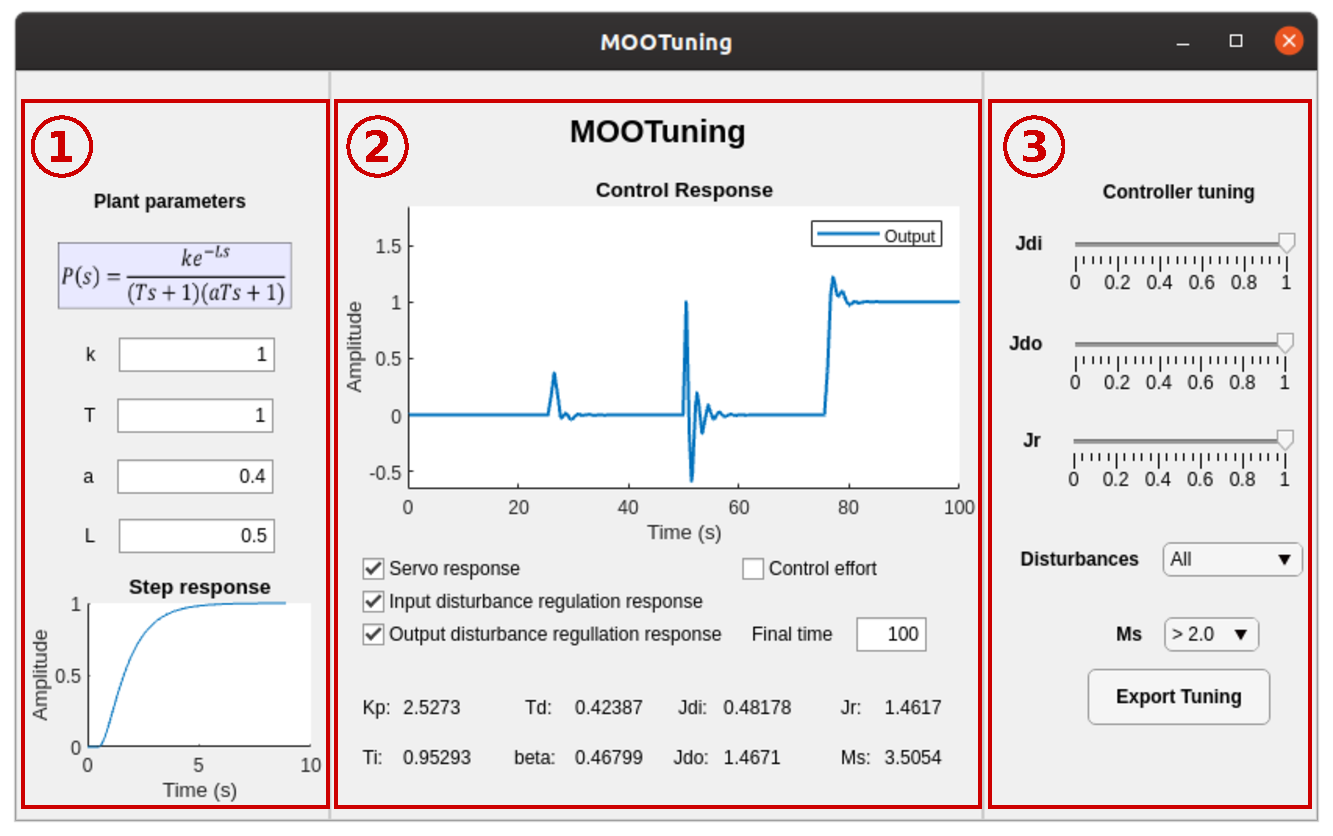
\includegraphics[width=0.8\columnwidth]{Ch6MOOTuningParts}
	\caption{Interface of MOOTuning for PID parameter selection.}
	\label{fig:Ch6MOOTuningParts}
\end{figure}
Figure~\ref{fig:Ch6MOOTuningParts}. It has three main components:
\begin{enumerate}
	\item Plant parameters input section
	\item Results section
	\item Tuning section
\end{enumerate}
%
The plant parameters input section is used to enter the parameters of the model of the plant. The expected model is an \gls{soptd}, but the value of $a$ can be set to zero, given the option to have also a \gls{foptd} model. However, it is necessary to have a normalized delay time larger than $0.1$. The tool warns the user when an invalid value is entered (as a negative time constant for example). When any of these parameters are changed, the step response plot at the bottom is automatically updated.

The second section shows the user the results of the selected tuning. The main component is a figure where the closed-loop response is plotted for the selected sources of disturbance: \textit{Servo response} is the closed-loop response to a setpoint step change, \textit{Input disturbance regulation response} plots the closed-loop response to a step change at the input of the plant and \textit{Output disturbance regulation response} plots the closed-loop response to  step change at the output of the plant. The control effort can be plotted as well in the same graph.

At the bottom of the second section, the results of the controller parameters, the value of the cost function and the value of the maximum sensitivity are presented with the given tuning. These are updated every time the user makes a change in the third section of the tool.

The last section of the tool is the Tuning section. Here, the user is presented with a series of ``decision choices'' that defines which of the points of the front is selected as the final tuning. The sliders at the top represents the \textit{allowed degradation} of the function with respect to the optimal point. A value of zero means that the lowest value of the cost function is desired, while a value of 1 represents that the function can have any value (even its maximum value).

The tool select the function with the lowest allowed degradation as the main cost function. Then, it searches for a set of parameters that comply with all the degradation limits set by the user, that also has the lowest possible value of the main function. As it can be seen, this tool let the user select the desired value from the Pareto, without the need to plot the front.

The user has also the ability to select if all the cost function need to be used for the tuning, or if only the input disturbance and the setpoint change are considered. Finally, the user can select different values of Maximum Sensitivity, to set the robustness of the closed-loop system. The \textit{Export Tuning} button let the user to copy the values of the tuning and export them as an structure to the \matlab{} workspace.

Of course, it may be possible that the user selects a set of values for $J_{di}$, $J_{do}$ and $J_r$ that do not correspond to a Pareto point. In that case, the tool shows a window indicating that the current selection is not feasible. This window is shown in %
%
\begin{figure}[tb]
	\centering
	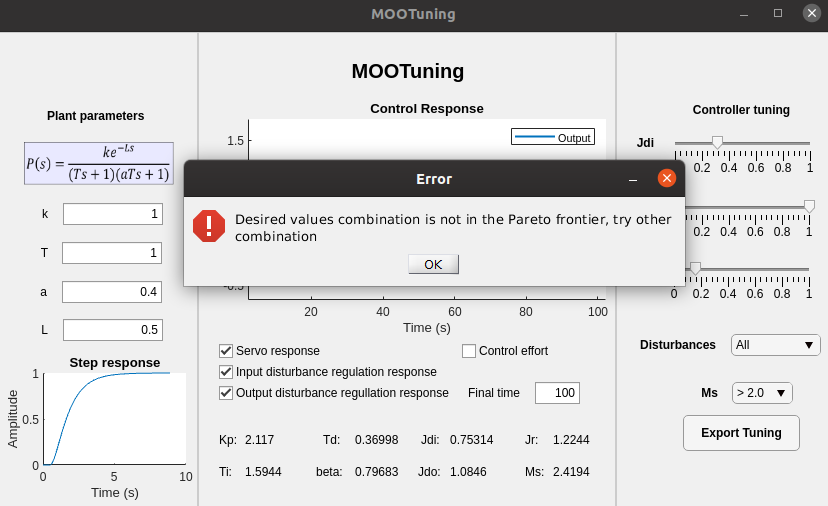
\includegraphics[width=0.8\columnwidth]{Ch6MOOTuning}
	\caption{Error raised if the desired point lies outside the Pareto front.}
	\label{fig:Ch6MOOTuning}
\end{figure}
%
Figure~\ref{fig:Ch6MOOTuning}. The user than can relax the allowed degradation of the cost function to be able to find the appropriate tuning. The figures can be saved using the standard \matlab{} methods.

\subsection{Example using MOOTuning}
\label{sec:MOOTuningExample}
To do.